\chapter{Bandpass Filter} \label{ch:bandpassFilter}

In this chapter, we introduce and analyze a bandpass filter for dispersive qubit measurement.
First, we explain the rationale for the bandpass filter and compare it qualitatively to existing systems.
Next, we quantitatively analyze the bandpass filter, arriving at a relation between the response time of the filtered measurement system and the coherence of the qubit.
The analysis is corroborated with numerics.
We then use the results of the analysis to choose circuit parameters.
We then determine the physical geometry of the hardware elements needed to achieve the desired circuit parameters.
Finally, we describe the fabrication steps used to build the device.

\section{Rationale}

As described in Chapter \ref{ch:MeasuringQubitState}, research at Yale demonstrated that adding a filter to the dispersive measurement system improves the qubit $T_1$ \cite{Reed:filter2010}.
A block diagram of the circuit used in that and similar experiments is shown in Fig.\,\ref{Fig:ch:bandpassFilter:sec:rationale:notchTopology}\,a.
The experiment in Ref. \cite{Reed:filter2010} used a single qubit, but other experiments with similar technology used multiple qubits all attached to a common resonator \cite{DiCarlo:algorithms2009, Majer:bus2007, Reed:errorCorrection2012}.
We have accordingly added a second qubit and filter to the diagram to guide the discussion of how the filter system might be extended for use in a multi-qubit system.

The filter, placed in series with the shared resonator, protected the qubit by introducing a notch at the qubit's frequency, as shown in Fig.\,\ref{Fig:ch:bandpassFilter:sec:rationale:notchTopology}\,b.
This prevented spontaneous emission of energy from the qubit into the environment, but the design has some important limitations.
First, the notch filter protects the qubit over a narrow band of frequency.
This precludes use of high fidelity logic gates based on dynamic tuning of the qubit frequency \cite{Barends:gates2014}, as changing a qubits' frequency would bring it out of the protected notch and lower its coherence time.
It may be possible in principle to use multiple notch filters arranged in series to create a protected ``bucket'' as shown by the dotted line in Fig.\,\ref{Fig:ch:bandpassFilter:sec:rationale:notchTopology}\,b, but this would require many filters, each of which requires large on-chip area.
Second, the measurement resonator itself was connected in series with the microwave feed line.
This precludes use of multiple resonators, because two detuned resonators in series act as an open circuit.
Therefore each qubit in a multi-qubit system is connected to a single resonator.
The requires that the states of the multi-qubit system be uniquely mapped into the phase space of a single resonator mode, as shown in Fig.\,\ref{Fig:ch:bandpassFilter:sec:rationale:notchTopology}\,c.
The number of states to distinguish grows exponentially with the number of qubits.
Therefore, in a large system, phase space and frequency crowding would lead to measurement cross-talk and/or reduced visibility.\footnote{This crowding effect has actually been used to directly measure two qubit parity with a single resonator mode \cite{Chow:jointReadout2010}.}

\begin{figure}
\begin{centering}
\includegraphics[width=\columnwidth]{notchTopology.pdf}
\par\end{centering}
\caption{Notch filter circuit topology. a) A single resonator (blue) interrupts the microwave feed line in series. Several qubits are coupled in parallel to the single resonator mode. Notch filters (green and brown) on the resonator output protect the qubits against from emission. b) The resonator mode produces a strong transmission peak, while the notch filters produce dips. The qubit frequencies are matched to the filters. c) The qubit states are distinguished in the amplitude-phase plane for the resonator mode.}
\label{Fig:ch:bandpassFilter:sec:rationale:notchTopology}
\end{figure}

We addressed these issues by inverting the role of the filter.
Rather than use filter notches to suppress emission only at the qubit frequencies, we use a bandpass filter to suppress emission everywhere except at the measurement frequency.
The starting point for our design is a set of measurement resonators connected in parallel with the microwave line, as shown in Fig.\,\ref{Fig:ch:bandpassFilter:sec:rationale:bandpassTopology}.
This circuit topology is standard in microwave kinetic inductance detector (MKID) systems used for astrophysical observation, and was demonstrated for qubit systems in previous experiments \cite{Chen:readout2012, Barends:XMon2013}.
This topology addresses the issue of measurement cross-talk and phase space crowding by using a separate measurement resonator for each qubit.
We then essentially replace a section of the drive line with a $\lambda/4$ resonator, which acts as a filter.
The resonators are connected in parallel to the filter.
The filter is of the bandpass type, with high transmission over a band encompassing all of the measurement resonators, and low transmission elsewhere, as shown in Fig.\,\ref{Fig:ch:bandpassFilter:sec:rationale:bandpassTopology}\,b.
The qubits, sitting outside the pass band of the filter are protected from the emission into the environment.
Note that, because the filter's stop band extends indefinitely at low frequencies, multiple qubits are protected simultaneously, and dynamic frequency tuning of the qubits is possible while keeping the qubits protected.
Frequency crowding of the measurement resonators within the filter pass band will be an issue in larger systems, but this can be addressed by connecting several filter circuits in parallel to a common microwave line.

\begin{figure}
\begin{centering}
\includegraphics[width=\columnwidth]{bandpassTopology.pdf}
\par\end{centering}
\caption{Bandpass filter circuit topology. a) Several measurement resonators (blue) connect in parallel to the microwave feed line, each one connected to a single qubit. The filter (green) is embedded directly into the feed line. b) The measurement resonators, which produce dips in the transmission spectrum, are all placed within the filter pass band. The qubits sit out of the pass band and are protected from emission. c) Each resonator's amplitude and phase contains the information of only one qubit state.}
\label{Fig:ch:bandpassFilter:sec:rationale:bandpassTopology}
\end{figure}

In the bandpass filter circuit, there is really no intrinsic difference between the role of the filter and the role of the measurement resonator.
Comparing Fig.\,\ref{Fig:ch:bandpassFilter:sec:rationale:bandpassTopology}\,a to Fig.\,\ref{Fig:resonatorMeasurement}, we see that filter is in a sense just another pole in the measurement resonator.
This idea is brought forth in Fig.\,\ref{Fig:lumpedModel}, which will be analyzed in depth in the following analysis.

\subinputfrom{../../Theory/DispersiveReadout/purcell/derivation-2/}{analysis}
\subinputfrom{../../Theory/DispersiveReadout/purcell/}{numerics}
\subinputfrom{./}{circuitParameters}
\subinputfrom{./}{device}
